
\chapter{Vergelijking IPv4 met IPv6}
\label{ch:h2}

In dit hoofdstuk zal er dieper worden ingegaan op de verschillen tussen beide protocollen, specifiek de vorming van de headers. Welke aanpassingen er werden gemaakt naar aanleiding van het nieuwe internet protocol en eveneens de mogelijke effecten deze verschillen kunnen hebben. Hiermee zal er een duidelijk zicht gegeven worden waarmee er juist rekening wordt gehouden naar aanleiding van de ontwikkeling van IPv6. Dit hoofdstuk bevat dus een voorstudie naar aanleiding van de overschakeling naar IPv6.

\section{Header van IPv4 en IPv6}

Onderstaande figuur geeft een duidelijke weergave van de IPv4 en IPv6 headers. Beide hebben een duidelijk verschil naar gelang de inhoud, aantal velden en aantal gebruikte bits. Op het eerste zicht is er te zien dat een IPv6 header een eenvoudiger overzicht handhaaft. Door het minder aantal velden in de header tegenover die van IPv4. Dit maakt van IPv6 een gestroomlijnder protocol en is zo efficiënter om af te handelen. Nog een voordeel hiervan is dat een IPv6 header een vaste 40 bits header bevat in vergelijking met IPv4, waarbij een IPv4 header gebruik maakt van een variabele lengte voor zijn header. Verder in dit hoofdstuk worden de verschillende velden met elkaar vergeleken.


\begin{figure}
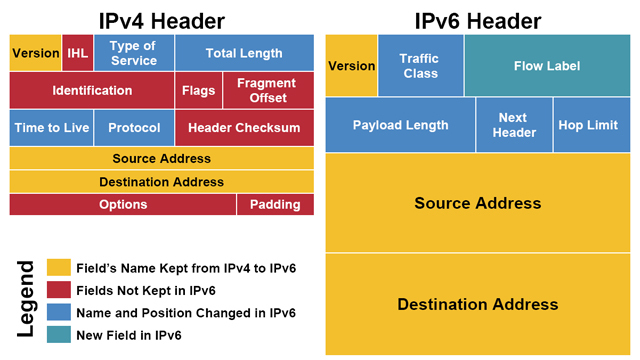
\includegraphics[width=\textwidth,height=\textheight,keepaspectratio]{vergelijking.jpg}
\centering
\caption{Vergelijking IPv4 header en IPv6 header \autocite{4vs6}}
\centering
\end{figure}

\subsection{Version Field}

Zowel IPv4 als IPv6 begint met een versie veld. Dit veld bevat de versie van het gebruikte internet protocol. Bij IPv4 zal dit de waarde 4 opleveren en voor IPv6 zal dat de waarde 6 zijn \autocite{Graziani2017}.

\subsection{IPv4 Internet Header Length (IHL) Field}

IHL is de lengte van de IPv4 header in 32-bit woorden, met optionele velden. In feite toont dit het einde van de IPv4 header en het begin van de data of payload. De minimumwaarde van dit veld is 5. Dit betekent 5 keer 32-bit woorden of 160 bits, in octetten is dit 20 bytes. Dit komt dus overeen met de minimumwaarde van een IPv4 header zonder optionele velden. Deze optionele velden kunnen de lengte van het IHL tot een maximum van 60 bytes brengen. In vergelijking met IPv6, bestaat dit veld niet meer in de nieuwe header. De reden waarom dit veld in meer van noodzaak is in de header, is omdat een IPv6 header een vaste lengte gebruikt namelijk 40 bytes. Dit zorgt ervoor dat het behandelen veel efficiënter te pas kan gaan. Ook maakt IPv6 gebruik van optionele velden maar deze hebben geen invloed op de lengte, dit behoudt de vaste lengte van de header \autocite{Graziani2017}.

\subsection{IPv4 Type of Service (ToS) en IPv6 Traffic Class Fields}

Type of Service in IPv4 en Traffic Class Fields zijn in principe dezelfde velden. Juist werd de naamgeving hiervan aangepast in IPv6. Beiden worden gebruikt om te preciseren welke soort behandeling het pakket juist zal krijgen van routers. Deze informatie zal helpen om de functies van Quality of Service (QoS) te leveren door verschillende graden van precedentie aan te bieden. Wanneer er meerdere pakketten verstuurd worden vanuit dezelfde interface dan kan de waarde in dit veld een hulp bieden voor zowel de behandeling van pakket als voor de volgorde waarin de pakketten verstuurd worden \autocite{Graziani2017}.

\subsection{IPv6 Flow Label Field}

Het flow label field wordt gebruikt om alle pakketten binnen dezelfde stroom/flow te helpen identificeren en ervoor te zorgen dat alle pakketten dezelfde behandeling krijgen van de IPv6-routers. Routers houden de individuele pakketstromen bij. Omdat de routers niet onafhankelijk de header van elk pakket hoeven te verwerken, worden deze multipakket flows efficiënter verwerkt. Echter zijn er niet veel implementaties die rekening houden met flow label. Behalve Equal Cost Multi-Path (ECMP) en Server Load Balancing (SLB). Als een flow label de waarde 0 bevat dan betekent dit dat er met het verkeer geen rekening gehouden zal worden met een flow \autocite{Graziani2017}.

\subsection{IPv4 Total Length Field, IPv6 Payload Length Field en IPv6 Jumbograms}

Het IPv4 Total Length Field is de totale lengte van het IPv4 pakket, dit wordt uitgemeten in bytes, en bevat zowel de header als de data. Het veld is een 16-bit veld en dus een maximum grootte van een IPv4 pakket is 65535 bytes. De meeste IPv4 pakketten zijn dus ook kleiner van grootte \autocite{Graziani2017}.

Het IPv6 Payload Length Field is een 16-bit veld dat de lengte in bytes van het data deel van een IPv4-pakket. Echter telt de lengte van de IPv6 header hierin niet mee en bevat het enkel de data en IPv6-extensies. Als het pakket dus extensies bevat zullen deze hierin ook meegeteld worden. Extensies worden beschouwd als een deel van de payload \autocite{Graziani2017}.

Beiden zijn met elkaar te vergelijken, behalve voor één belangrijk verschil. In het IPv4 Total Length Field bevat het de totale lengte van een IPv4-pakket, zowel data als header. Bij het IPv6 Payload Length Field is dit enkel het totaal aantal bytes van de data of payload, de header wordt hierin niet meegerekend. Daarom kan de lengte bij IPv4 verschillen door gebruik te maken van optionele velden waarbij IPv6 een vaste lengte heeft van 40 bytes \autocite{Graziani2017}.

Zoals eerder vermeld geweest, IPv4 Total Length is een 16-bit veld dat een maximum pakket grootte van 65355 bytes heeft. Deze pakketten zullen deze grootte haast nooit halen wegens de maximum transmission unit (MTU). IPv4 heeft geen optie om deze theoretische grootte te overschrijden. Daarentegen kan IPv6 zijn maximum payload wel overschrijven. Dit type van pakket wordt dan een jumbogram genoemd. Een jumbogram is een IPv6-pakket dat een grotere payload van 65535 bytes bevat. Jumbogrammen gebruiken de Jumbo Payload optie in de Hop-by-Hop extensie header. De Jumbo payload optie gebruikt een veld van 32-bit lengte groot om het verzenden van IPv6-pakketten tussen de 65536 en 4294967295 bytes toe te laten. Deze jumbogrammen worden het vaakst gebruikt bij connecties tussen supercomputers \autocite{Graziani2017}.

\subsection{IPv4 en IPv6 MTU's}

De meeste transmissie linken gebruiken een maximum pakketlengte gekend als een MTU (maximum transmission unit). Een MTU bij IPv4 en IPv6 is de totale lengte van een pakket inclusief de header \autocite{Graziani2017}. 

Echter is het nodig dat elke node de mogelijkheid heeft om een Ipv4 pakket te versturen van 68 bytes zonder verdere fragmentatie. Dit komt omdat een Ipv4 header de grootte van 60 bytes kan bevatten in lengte, waardoor er nog 8 bytes overblijven voor de payload. Daarom moet de payload een Ipv4 fragment zijn. Anders moet de payload header informatie toegevoegd krijgen voor een ander protocol, waardoor het groter dan 8 bytes zal worden. Elke IPv4 eindbestemming van het Ipv4 pakket moet een IPv4 pakket van 576 bytes kunnen ontvangen, dit kunnen ook alle fragmenten van een pakket zijn \autocite{Graziani2017}.

Bij IPv6 is het nodig dat elke link een minimum MTU van 1280 bytes heeft, met een aangeraden MTU van 1500 bytes. In vergelijk met het IPv4 protocol is dit 68 bytes \autocite{Graziani2017}.

\subsection{IPv4 Framgmentation}

Het IPv4 protocol werd eerder ontwikkeld voor een breed spectrum van transmissielinks. Als de router een IPv4 pakket ontvangt dat groter is dan de MTU van de uitgaande interface dan kan het pakket gefragmenteerd worden afhankelijk van de header van het pakket. Het kan voorvallen dat een pakket al gefragmenteerd, in meerdere pakketten, werd verzonden door de verzender. Als de finale ontvanger alle pakketten ontvangt, dan is het zijn taak om deze terug te zetten in het originele IPv4 pakket \autocite{Graziani2017}.

Fragmentatie deelt dus IPv4 pakketten in kleinere delen zodat deze kunnen doorgestuurd worden op een link dat niet de volledige grootte van het originele pakket kon verzenden. Het bestemmende apparaat heeft als taak deze ontvangen pakketten terug om te vormen naar het originele pakket. Het IPv4 Identification, Flags en Fragment Offset velden worden gebruikt om het pakket op te delen en terug samen te voegen \autocite{Graziani2017}. 

Identification veld is 16 bits groot. Elk IPv4 pakket heeft een uniek veld in het 16 bit Identification veld. Als een IPv4 pakket wordt opgesplitst in delen dan helpt dit veld om de gefragmenteerde pakketten terug samen te voegen voor de ontvanger \autocite{Graziani2017}.

Flags veld is een veld dat de grootte heeft van 3 bits. De eerste bit is 0, dit geeft aan of het gereserveerd is of niet. De tweede bit is bekend als de DF (don’t fragment) bit. Als deze de waarde 1 heeft toont dit aan dat het pakket niet gefragmenteerd is. De laatste, derde, bit is de more fragments flag. Deze bit is gebruikt om aan te tonen of dit pakket het laatste pakket is of niet. Als deze de waarde 1 heeft dan is dit pakket niet het laatste en volgen er nog. 0 geeft aan dat dit het laatste pakket is. Als een IPv4 pakket niet gefragmenteerd is dan zal deze vlag de waarde 0 bevatten \autocite{Graziani2017}.

Fragment Offset veld is een veld van 13 bits lang. Als een IPv4 pakket is gefragmenteerd dan toont dit veld aan waar het pakket gepositioneerd is en waar de data komt in delen van 8 octetten, 64 bits. De ontvanger krijgt hierdoor een beeld van waar het pakket komt tussen alle andere pakketten. Als het pakket niet gefragmenteerd is zal deze de waarde 0 hebben \autocite{Graziani2017}.

\subsection{IPv6 Fragmentation: IPv6 Source only}

Een IPv6 router zal geen fragmentering toepassen op een pakket, zoals bij IPv4 wel het geval is, enkel als het de zender is van het pakket. Zoals te zien op de afbeelding is er in de IPv6 header geen plaats gemaakt voor de velden die IPv4 gebruikt om te fragmenteren \autocite{Graziani2017}.

Als een IPv6 router een pakket ontvangt dat groter is dan de MTU uitgaande interface, dan zal de router simpelweg het pakket droppen en zal een ICMPv6 (Internet Control Message Protocol version 6) Packet Too Big bericht terug verzenden naar de zender van het pakket. Het Packet Too Big bericht bevat de MTU grootte van de link in bytes zodanig dat de zender van het pakket zijn grootte kan aanpassen en het pakket terug kan verzenden \autocite{Graziani2017}.

De data wordt vaak verzonden in series van pakketten, ook wel een packet train genoemd. Hoe groter deze pakketten zijn, hoe minder pakketten er zullen verstuurd moeten worden. Daarom is het aangeraden om de grootte zo hoog mogelijk te maken zodat alle links, van zender naar ontvanger, deze ondersteunen. Dit wordt ook de Path MTU (PMTU) genoemd. Hiervoor kan een apparaat een PMTU Discovery doen om de laagste MTU link te achterhalen \autocite{Graziani2017}.

\subsection{IPv4 Protocol en IPv6 Next Header Fields}

Het IPv4 Protocol veld toont het protocol aan dat gebruikt wordt in de data portie van het IPv4 pakket. Hiervoor heeft IPv6 een gelijkaardig veld, het Next Header veld, dat aantoont welk type header er volgt achter de algemene IPv6 header. Ook al lijkt het gelijkaardig met het IPv4 veld, toch zijn er enkele verschillen tussen beiden \autocite{Graziani2017}.

Dezelfde waarden die gebruikt worden in het IPv4 Protocol veld zijn terug te vinden in het IPv6 Next Header veld, buiten dat er bij IPv6 nog extra waarden mogelijk zijn. De meest voorkomen waarde voor beiden is voor TCP de waarde 6 en voor UDP 17 \autocite{Graziani2017}.

Als er enkel een IPv6 header is en geen extra header meer volgt, dan zal het IPv6 Next Header veld de waarde van het protocol weergeven dat wordt gebruikt in de data portie van het IPv6 pakket. Dit is dus hetzelfde voor het IPv4 Protocol veld \autocite{Graziani2017}.

\subsection{IPv4 Time To Live (TTL) en IPv6 Hop Limit Fields}

De IPv4 Time To Live (TTL) en IPv6 Hop Limit velden zorgen ervoor dat pakketten niet eindeloos blijven rondgaan in netwerken, zoals routingloops. Deze velden worden steeds verminderd door 1 als het pakket een router passeert. Als het veld de waarde 0 bereikt dan wordt het pakket weggegooid en een ICMPv4 of ICMPv6 Time Exceeded bericht verstuurd naar de zender van het pakket \autocite{Graziani2017}. 

Van IPv4 naar IPv6, was het TTL veld verandert naar het Hop Limit veld. Het IPv4 TTL veld was eigenlijk bedoelt om het maximum aantal tijd dat het pakket mag ronddolen in een netwerk en niet het aantal hops met routers. Deze tijd wordt berekend in seconden. Het maximum is 255 seconden of 4.25 minuten. In plaats van deze tijd te berekenen gaan de routers het IPv4 TTL veld verminderen met 1, hierdoor worden het aantal van hops aangekaart \autocite{Graziani2017}.

\subsection{Checksums: IPv4, TCP en UDP}

Een checksum in de IPv4 header dient ervoor om na het versturen van pakketten deze te controleren op corrupte data. Dit is een 16-bit checksum die zich focust op de IPv4 header. Elke router die dit pakket passeert zal de berekening doen van de checksum en controleren. Als deze dan gefaald of fout is zal de router het pakket verwijderen \autocite{Graziani2017}.

In IPv6 is er geen checksum in de IPv6 header. De checksum is er bewust uitgelaten omdat layer 2 data link technologie, zoals ethernet, een eigen checksum en error controle hebben. Alsook TCP en UDP hebben hun eigen checksums. Dit maakt een extra checksum op layer 3 niveau overbodig en redundant \autocite{Graziani2017}.

Omdat er geen checksum is toegevoegd in IPv6 zal de UDP checksum wel verplicht zijn bij IPv6, wat bij IPv4 niet het geval is. Dit veld dient er toe om de betrouwbaarheid van de UDP header en data te waarborgen. Bij het TCP protocol is zowel bij IPv6 als bij IPv4 de checksum een vereiste \autocite{Graziani2017}.

Checksums worden gebruikt op verschillende layers door verschillende protocollen. Een checksum zal dus controleren op mogelijk fouten die zijn opgelopen tijdens het verzenden van de data. Elk transport laag of andere bovenlaag protocol dat een IPv4 adres bevat in de berekening van de checksum moet veranderd worden voor het IPv6 te kunnen gebruiken. Deze wijziging is nodig voor het 128-bit IPv6 adres \autocite{Graziani2017}.

Wanneer TCP of UDP verzonden word over IPv6, dan bevat de checksum enkele velden namelijk IPv6 bronadres, IPv6 bestemmingsadres, de payload van de bovenlaag en de IPv6 next-header waarde \autocite{Graziani2017}.

Een wijziging aan zowel TCP als UDP voor het transporteren van IPv6 pakketten is dus nodig. Omdat beide checksums gebruik maken van de IPv6 adressen, is het dus nodig deze te herwerken voor het langere adres. Ook al zijn de adressen langer, de werkwijzen en berekeningswijze blijven dezelfde voor zowel IPv6 als IPv4 \autocite{Graziani2017}.

Bij IPv4 is er een checksum aanwezig in de header, dit maakt voor UDP de checksum overbodig. Bij IPv6 was de checksum vooral verwijdert om de snelheid van de verwerking te verbeteren. Daarom is het dus verplicht om bij TCP en UDP de checksum te gebruiken \autocite{Graziani2017}.

\subsection{IPv4 en IPv6 bronadres en bestemmingsadres velden}

Eén van de grootste veranderingen van IPv4 naar IPv6 is de lengte van het bron- en bestemmingsadres. De lengte van de adressen zijn van 32-bit adressen naar 128 bit-adressen veranderd in IPv6 \autocite{Graziani2017}. Enkele veranderingen zijn:

\begin{itemize}
    \item Het bronadres is altijd een unicast adres, bij IPv6 kan dit een link-local unicast, unique local unicast of unspecified unicast adres zijn
    \item Het bestemmingsadres kan een unicast, multicast, anycast of een broadcast adres zijn. Bij IPv6 is enkel het broadcast adres niet aanwezig
\end{itemize}
